\documentclass[../main]{subfiles}

\questiontrue
\solutiontrue


\begin{document}
    \ifquestion
    \section{Multiplayer Astronomy}
	
	
	Johannes Kleber travels to Asunción (25° 16' 55" S; 57° 38' 06" W; GMT: -4h) in Paraguay on February 21st to buy products for his astronomy store. In the past, he even bought two altazimuth telescopes, one of which he sold to Nill, his friend, and the other he kept for himself. Upon arrival, with nothing to do on a night, at 21h1min37s, he observes the sky and finds an interesting object at an altitude of 40°. At the same moment, he contacts Nill (who was in Imperatriz - Brazil (5° 31' 33" S; 47° 28' 33" W; GMT: -3h)) who coincidentally was also observing the object (both inaugurating their new telescopes). Nill tells Kleber that he observed the hour angle of the object was 1h15min. Excited by the discovery, they return to looking through their respective telescopes to find more information, but they realize that their telescopes were broken. Sad but curious, they think for a while, with the information exchanged earlier, and both conclude that the object is:
	
	\begin{itemize}
		\item Consider that the sidereal time in Greenwich on January 1st, 2021 at 00:00 is 6h43min28.5s.
		\item Consider the celestial chart below:
	\end{itemize}
	
	\fig{0.5}{tele80.PNG}
	
	\clearpage
    \fi
	
	\ifsolution
    \section{Multiplayer Astronomy}
	
	Let $\phi_K$ be Kleber's latitude and $h$ the altitude of the object, using the known relation between hour angle ($H$), declination ($\delta$), latitude ($\phi$), and altitude ($h$):
	
	$$\cos{H}=\sin{h}\sec{\delta}\sec{\phi}-\tan{\delta}\tan{\phi}$$
	
	Given the latitude and altitude of the object, the hour angle is needed to find the declination. For this, we will use Nill's observation.
	
	The hour angle for Nill is $1h15min$. Considering the difference in longitude: $\Delta \lambda = \lambda_K-\lambda_L = -57^\circ 38' 06''-(-47^\circ 28' 33'')=-10^\circ9'33''=-40min38.2s$
	
	Thus: $H_K=H_L+\Delta \lambda = 1h15min - 40min38.2s = 34min21.8s = 8^\circ35'27''$. Substituting the values:
	
	$$\cos{8^\circ35'27''}=\sin{40^\circ}\sec{\delta}\sec{-25^\circ 16' 55''}-\tan{\delta}\tan{-25^\circ 16' 55''}$$
	
	Define: $a=\tan{25^\circ 16' 55''}=0.4723$; $b=\sin{40^\circ}\sec{25^\circ 16' 55''}=0.7109$ and $c = \cos{8^\circ35'27''}=0.9888$. Remembering that $(\sec{\theta})^2=(\tan{\theta})^2+1$, and letting $\tan{\delta}$ be $x$:
	
	$$ax+b\sqrt{x^2+1}=c$$

	$$x^2+1=\left(\frac{c}{b}-\frac{a}{b}x\right)^2$$
	
	Define $\frac{c}{b}=C=1.3909$ and $\frac{a}{b}=A=0.6644$:
	
	$$(A^2-1)x^2 -2ACx + C^2-1=0$$
	
	$$-0.5586x^2-1.8481x+0.9346=0$$
	
	Solving for $x$:
	
	$$x=\tan{\delta}=\frac{1.8481\pm 2.346}{-1.1172}=-1.6542 \pm 2.1$$

	Finally, we find two values:

	$$\delta_1 \approx 24^o$$

	$$\delta_2 \approx -75^o$$
	
	\begin{figure}[htpb]
	  \centering

    \tikzset{every picture/.style={line width=0.75pt}} %set default line width to 0.75pt        

    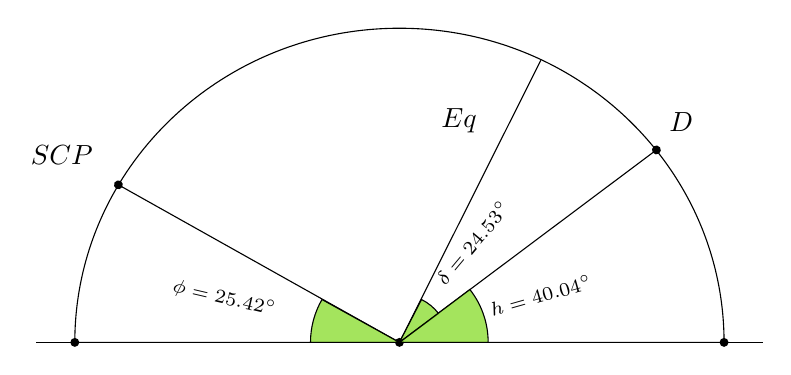
\begin{tikzpicture}[x=0.75pt,y=0.75pt,yscale=-1.2,xscale=1.2]
      %uncomment if require: \path (0,408); %set diagram left start at 0, and has height of 408

      %Straight Lines [id:da8600436790759003] 
      \draw    (184,282.34) -- (475.67,282.34) ;
      %Shape: Pie [id:dp2754682048797614] 
      \draw   (199.5,282.34) .. controls (199.5,282.34) and (199.5,282.34) .. (199.5,282.34) .. controls (199.5,212.68) and (257.85,156.21) .. (329.83,156.21) .. controls (401.81,156.21) and (460.17,212.68) .. (460.17,282.34) -- (329.83,282.34) -- cycle ;
      %Straight Lines [id:da855555142754068] 
      \draw    (386.6,169.08) -- (329.83,282.34) ;
      %Straight Lines [id:da29223282098135295] 
      \draw    (460.17,282.34) -- (329.83,282.34) ;
      \draw [shift={(329.83,282.34)}, rotate = 180] [color={rgb, 255:red, 0; green, 0; blue, 0 }  ][fill={rgb, 255:red, 0; green, 0; blue, 0 }  ][line width=0.75]      (0, 0) circle [x radius= 1.34, y radius= 1.34]   ;
      \draw [shift={(460.17,282.34)}, rotate = 180] [color={rgb, 255:red, 0; green, 0; blue, 0 }  ][fill={rgb, 255:red, 0; green, 0; blue, 0 }  ][line width=0.75]      (0, 0) circle [x radius= 1.34, y radius= 1.34]   ;
      %Straight Lines [id:da7115912008500032] 
      \draw    (433,205.08) -- (329.83,282.34) ;
      \draw [shift={(433,205.08)}, rotate = 143.17] [color={rgb, 255:red, 0; green, 0; blue, 0 }  ][fill={rgb, 255:red, 0; green, 0; blue, 0 }  ][line width=0.75]      (0, 0) circle [x radius= 1.34, y radius= 1.34]   ;
      %Straight Lines [id:da31496157698401706] 
      \draw    (199.5,282.34) -- (329.83,282.34) ;
      \draw [shift={(199.5,282.34)}, rotate = 360] [color={rgb, 255:red, 0; green, 0; blue, 0 }  ][fill={rgb, 255:red, 0; green, 0; blue, 0 }  ][line width=0.75]      (0, 0) circle [x radius= 1.34, y radius= 1.34]   ;
      %Straight Lines [id:da8857795102828852] 
      \draw    (217,219.08) -- (329.83,282.34) ;
      \draw [shift={(217,219.08)}, rotate = 29.28] [color={rgb, 255:red, 0; green, 0; blue, 0 }  ][fill={rgb, 255:red, 0; green, 0; blue, 0 }  ][line width=0.75]      (0, 0) circle [x radius= 1.34, y radius= 1.34]   ;
      %Shape: Pie [id:dp0007732956610952968] 
      \draw  [fill={rgb, 255:red, 132; green, 218; blue, 36 }  ,fill opacity=0.74 ] (294.13,282.34) .. controls (294.13,282.34) and (294.13,282.34) .. (294.13,282.34) .. controls (294.13,276.08) and (295.81,270.21) .. (298.74,265.13) -- (329.83,282.34) -- cycle ;
      %Shape: Pie [id:dp21553069833897842] 
      \draw  [fill={rgb, 255:red, 132; green, 218; blue, 36 }  ,fill opacity=0.74 ] (338.71,265.13) .. controls (341.4,266.47) and (343.74,268.4) .. (345.55,270.75) -- (329.83,282.34) -- cycle ;
      %Shape: Pie [id:dp2399716727588157] 
      \draw  [fill={rgb, 255:red, 132; green, 218; blue, 36 }  ,fill opacity=0.74 ] (358.12,261.11) .. controls (362.72,266.99) and (365.46,274.35) .. (365.46,282.34) -- (329.83,282.34) -- cycle ;

      % Text Node
      \draw (345.6,187.48) node [anchor=north west][inner sep=0.75pt]    {$Eq$};
      % Text Node
      \draw (180.8,202.08) node [anchor=north west][inner sep=0.75pt]    {$SCP$};
      % Text Node
      \draw (437.2,189.08) node [anchor=north west][inner sep=0.75pt]    {$D$};
      % Text Node
      \draw (239.1,254.81) node [anchor=north west][inner sep=0.75pt]  [font=\scriptsize,rotate=-13.24]  {$\phi =25.42^{\circ }$};
      % Text Node
      \draw (364.3,265.38) node [anchor=north west][inner sep=0.75pt]  [font=\scriptsize,rotate=-344.13]  {$h=40.04^{\circ }$};
      % Text Node
      \draw (342.06,256.29) node [anchor=north west][inner sep=0.75pt]  [font=\scriptsize,rotate=-310.05]  {$\delta =24.53^{\circ }$};


    \end{tikzpicture}
	  \caption{Representation of the geometry and the position of the points on the celestial sphere}
	  \label{fig:astrogeo}
	\end{figure}

	Now think: since the hour angle is approximately $8^\circ$, the object is "almost" on the local meridian. Thus, from the previous diagram, we conclude that the value we should adopt is $\delta_1 = 24^\circ$:
	
	Knowing the declination of the object, we must now find its right ascension $\alpha$. For this, we will find the sidereal time $T_{L}$ of Leibniz at the time of observation, knowing that $T_{L} = H + \alpha$. Since at the beginning of the year the sidereal time at Greenwich was $\alpha_G$, the sidereal time at the longitude $\lambda_L$ of Imperatriz-MA was $T_L = \alpha_G + \lambda_L$: $T_L = 6h43min28.5s + (-3h9min54.2s) = 3h33min34.3s$.
	
	To determine the sidereal time at the time of observation, remember that there are two effects to be considered: the Earth's translation and the Earth's rotation, therefore:

	$$\Delta T_L = T_L - T_{L,0} = \frac{24h}{365.24}\Delta T_{days} + \frac{24h}{23.9447}\Delta T_{hours}$$
	
	For the time of the analysis: $\Delta T_{days} = 51.920 days$ and $\Delta T_{hours} = 22.027 hours$ (remember to add one hour when converting from Kleber's timezone to Leibniz's). Thus, we finally find that $T_L = 29h2min56.6s = 5h2min56.6s$. From there, we determine that $\alpha = 3h47min56.6s$. In the presented image, this corresponds to the following point: 
	
	\fig{0.5}{tele89.PNG}

	This means that the observed object was the \textbf{Pleiades (M45)}.
	\clearpage

	\fi
	
\end{document}
